\let\negmedspace\undefined
\let\negthickspace\undefined
\documentclass[journal]{IEEEtran}
\usepackage[a5paper, margin=10mm, onecolumn]{geometry}
%\usepackage{lmodern} % Ensure lmodern is loaded for pdflatex
\usepackage{tfrupee} % Include tfrupee package

\setlength{\headheight}{1cm} % Set the height of the header box
\setlength{\headsep}{0mm}     % Set the distance between the header box and the top of the text

\usepackage{gvv-book}
\usepackage{gvv}
\usepackage{cite}
\usepackage{amsmath,amssymb,amsfonts,amsthm}
\usepackage{algorithmic}
\usepackage{graphicx}
\usepackage{textcomp}
\usepackage{xcolor}
\usepackage{txfonts}
\usepackage{listings}
\usepackage{enumitem}
\usepackage{mathtools}
\usepackage{gensymb}
\usepackage{comment}
\usepackage[breaklinks=true]{hyperref}
\usepackage{tkz-euclide} 
\usepackage{listings}
% \usepackage{gvv}                                        
\def\inputGnumericTable{}                                 
\usepackage[latin1]{inputenc}                                
\usepackage{color}                                            
\usepackage{array}                                            
\usepackage{longtable}                                       
\usepackage{calc}                                             
\usepackage{multirow}                                         
\usepackage{hhline}                                           
\usepackage{ifthen}                                           
\usepackage{lscape}
\begin{document}

\bibliographystyle{IEEEtran}
\vspace{3cm}

\title{NCERT - 11.16.2.2.8}
\author{EE24BTECH11040 - Mandara Hosur}
% \maketitle
% \newpage
% \bigskip
{\let\newpage\relax\maketitle}

\renewcommand{\thefigure}{\theenumi}
\renewcommand{\thetable}{\theenumi}
\setlength{\intextsep}{10pt} % Space between text and floats


\numberwithin{equation}{enumi}
\numberwithin{figure}{enumi}
\renewcommand{\thetable}{\theenumi}

\textbf{Question:}\\
A die is thrown. Consider the following events: \\
$A$: A number less than 7 is obtained \\
$B$: A number greater than 7 is obtained \\
Find $\Pr\brak{AB}$.

\textbf{Theoretical Solution:}\\
The probability mass function (PMF) for throwing a fair six-sided die is:
\begin{align}
    P_X\brak{x} = \begin{cases}
        \frac{1}{6} & \text{for } x = 1, 2, 3, 4, 5, 6 \\
        0 & \text{otherwise}
    \end{cases}
\end{align}
The cumulative distribution function (CDF) gives the probability of rolling a number less than or equal to some integer $x$.
\begin{align}
    F_X\brak{x} = \Pr\brak{X \leq x} = \begin{cases}
        0 & \text{for } x < 1 \\
        \frac{x}{6} & \text{for } x = 1, 2, 3, 4, 5, 6 \\
        1 & \text{for } x > 6
    \end{cases}
\end{align}
Thus, the probability of event $A$ can be calculated as follows:
\begin{align}
    \Pr\brak{A} = F_X\brak{7} - P_X\brak{7} = 1 - 0 = 1
\end{align}
Similarly, the probability of event $B$ can also be calculated (using the axiom of Boolean Algebra $E+E^{\prime}=1$ for some event $E$ in the sample space):
\begin{align}
    \Pr\brak{B} = \Pr\brak{X > 7} = 1 - \Pr\brak{X \leq 7} = 1 - F_X\brak{7} \\
    \implies \Pr{B} = 1 - 1 = 0
\end{align}
$A$ and $B$ can be observed to be mutually exclusive events, as no number $x$ can be lesser than and greater than 7 at the same time.
Hence, we can say that:
\begin{align}
    \Pr\brak{AB} = 0
\end{align}

\textbf{Simulated Solution:} \\
Let $X_1$ be an indicator random variable of the event $A$. $X_1$ is defined as:
\begin{align}
	X_1 =
	\begin{cases}
		1 ,& A\\
		0 ,& A^\prime\\
	\end{cases}
\end{align}
Let $X_2$ be the indicator random variable of the event $B$. $X_2$ is defined as:
\begin{align}
	X_2 =
	\begin{cases}
		1 ,& B\\
		0 ,& B^\prime\\
	\end{cases}
\end{align}
Let $X_3$ be the indicator random variable of the event $AB$. $X_3$ is defined as:
\begin{align}
	X_3 =
	\begin{cases}
		1 ,& AB\\
		0 ,& \brak{AB}^\prime\\
	\end{cases}
\end{align}
The PMF of the random variable $X_1$ is:
\begin{align}
	P_{X_1}\brak{n} = \begin{cases}
		p_1 ,& n = 1 \\
		1 - p_1 ,& n = 0
	\end{cases}
\end{align}
The PMF of the random variable $X_2$ is:
\begin{align}
	P_{X_2}\brak{n} = \begin{cases}
		p_2 ,& n = 1 \\
		1 - p_2 ,& n = 0
	\end{cases}
\end{align}
The PMF of the random variable $X_3$ is:
\begin{align}
	P_{X_3}\brak{n} = \begin{cases}
		p_3 ,& n = 1 \\
		1 - p_3 ,& n = 0
	\end{cases}
\end{align}
where,
\begin{align}
	p_1 &= 1\\
	p_2 &= 0\\
	p_3 &= 0\\
\end{align}

Through the definitions made earlier:
\begin{align}
	\Pr\brak{A} = p_1 =1 \\
	\Pr\brak{B} = p_2 = 0\\
	\Pr\brak{AB} = p_3 = 0
\end{align}

\textbf{Conclusion:} \\
The probaility of the event $AB$ is:
\begin{align}
    \Pr\brak{AB}
\end{align}

\textbf{Plots:}
\begin{figure}[h]
	\centering
	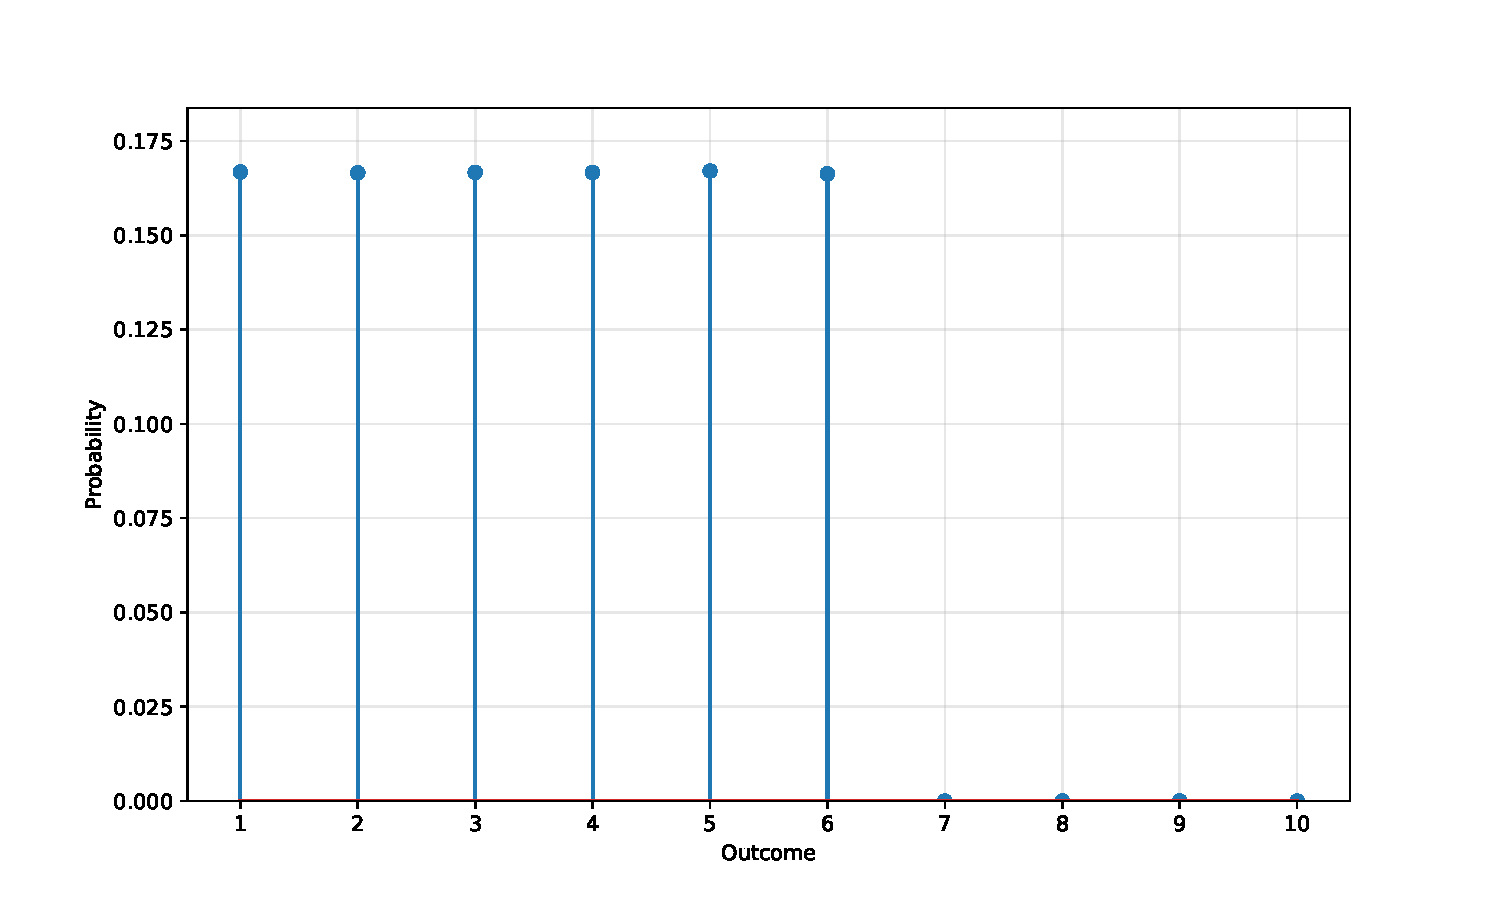
\includegraphics[width=\columnwidth]{figs/die_roll_pmf.pdf}
	\caption{Plot of PMF of die roll}
\end{figure}
\begin{figure}[h]
	\centering
	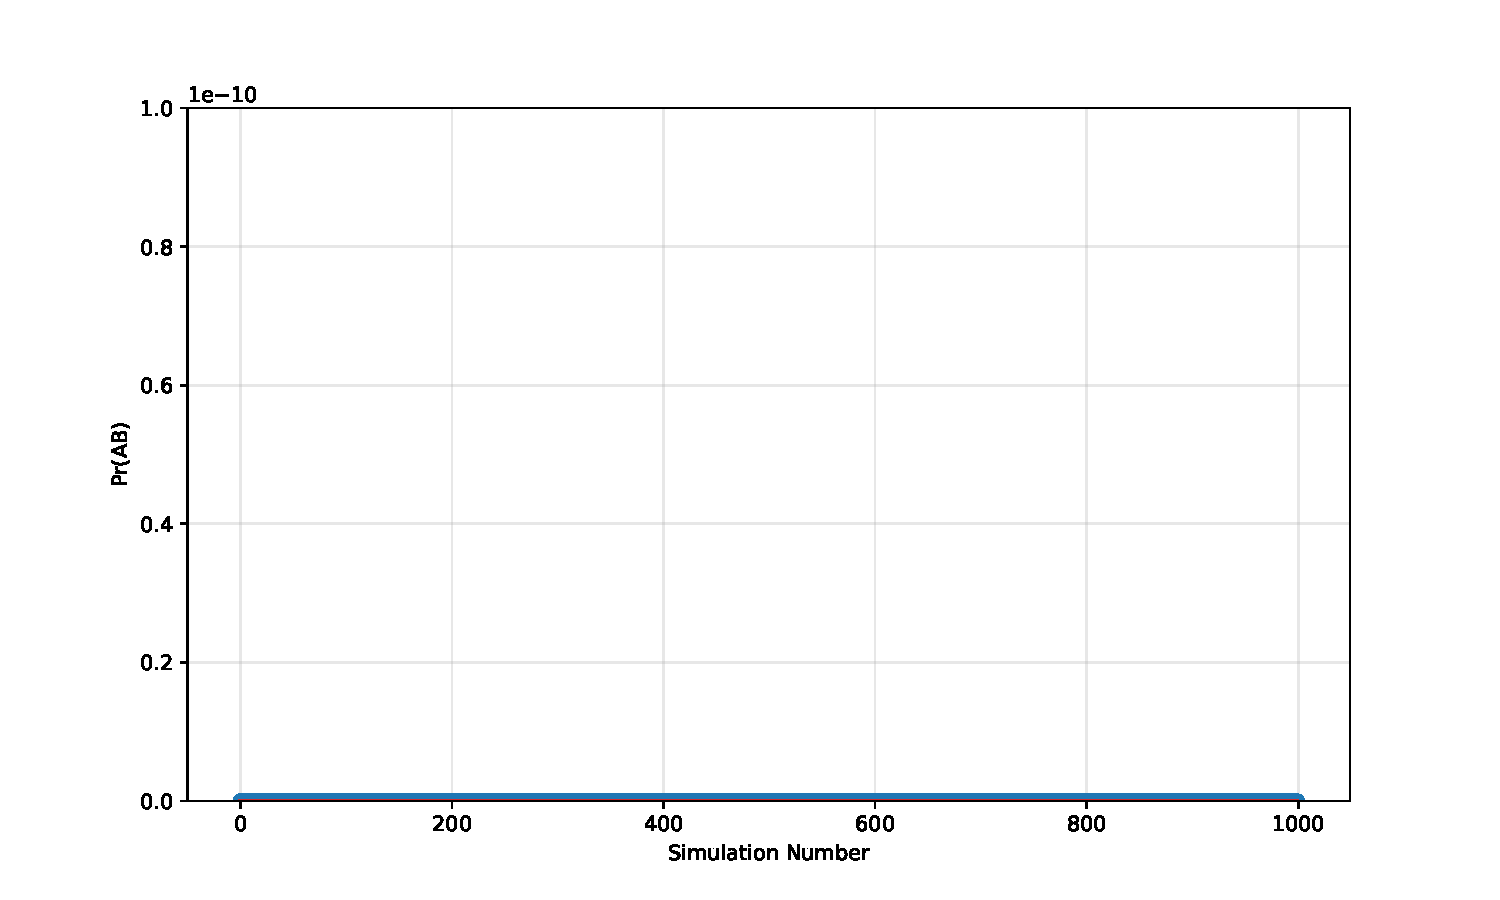
\includegraphics[width=\columnwidth]{figs/Pr_AB_simulation_results.pdf}
	\caption{Plot of PMF of $\Pr\brak{AB}$}
\end{figure}

\end{document}
